% Formal Methods at JPL - Klaus Havelund - September 2026 - 20 minutes

%\documentclass[10pt,xcolor=dvipsnames,xcolor=table,handout]{beamer}
\documentclass{beamer}

\title{Formal Methods at JPL}

\author{{\bf Klaus Havelund}\\
Jet Propulsion Laboratory\\
California Institute of Technology\\
%\vspace{1cm}
%{\scriptsize The research was carried out under a contract\\ with the National Aeronautics and Space Administration.}
}

\date[]{JPL --- September 2026}

% If you wish to uncover everything in a step-wise fashion, uncomment
% the following command:
%\beamerdefaultoverlayspecification{<+->}

\mode<presentation>
{
\usetheme{Madrid}
\setbeamercovered{transparent=5}
\setbeamertemplate{navigation symbols}{}
}

\PassOptionsToPackage{bookmarks=true,bookmarksopen=true,pdfborder={0 0 0},pdfhighlight={/N},linkbordercolor=[rgb]{0.5,0.5,0.5},implicit=false,hidelinks}{hyperref}
\usepackage[T1]{fontenc}   % so < > in \ttfamily render correctly, not as inverted marks
\usepackage{colortbl}      % \rowcolor in tabulars
\usepackage{cite}
\usepackage{amscd}
\usepackage{amsmath,amssymb,amsfonts}
\usepackage{cases}
\usepackage{commath}
\usepackage[hidelinks]{hyperref}
\usepackage{float}
\usepackage{forest}
\usepackage{hhline}
\usepackage{graphicx}

\usepackage{textcomp}
\usepackage{xcolor}
\usepackage{multirow}
\usepackage{tabularx,ragged2e}
\usepackage[skip=2pt]{caption}
\captionsetup[table]{skip=6pt}
\usepackage{subcaption}
\usepackage{multirow}
\usepackage{listings}
\usepackage{xcolor}
\usepackage{todonotes}
\usepackage{rotating}

\usepackage{booktabs} % For better table rules
\usepackage{threeparttable} % For table notes
\usepackage{multirow} % Required for merging rows
\usepackage{tabularx} % For adjustable-width columns
\usepackage{tabto}
\usepackage[most]{tcolorbox}
\usepackage{xcolor}
\usepackage{lipsum}
\usepackage{array}

% table spacing
\setlength{\tabcolsep}{8pt}  % column gap (default is 6pt)
\renewcommand{\arraystretch}{0.95}  % row height (default is 1.0)

\newcommand{\needsref}{\textsuperscript{*}}

\tcbset{
  user/.style={
    colback=blue!5!white,
    colframe=blue!75!black,
    fonttitle=\bfseries,
    title=User,
    sharp corners,
    boxrule=0.5pt,
    left=2mm, right=2mm, top=1mm, bottom=1mm,
  },
  agent/.style={
    colback=gray!10!white,
    colframe=black!60!white,
    fonttitle=\bfseries,
    title=Tool,
    sharp corners,
    boxrule=0.5pt,
    left=2mm, right=2mm, top=1mm, bottom=1mm,
  }
}

\newcommand\ipyt{\lstset{language=python}\lstinline}

\lstdefinestyle{matlab} {
        language=Matlab,
        backgroundcolor=\color[rgb]{0.95,0.95,0.92},
        commentstyle=\color[rgb]{0.13,0.55,0.13}\em,
        stringstyle=\color[rgb]{0.7,0,0},
        basicstyle=\ttfamily\scriptsize}

\lstset{style=matlab,
        captionpos=b,
        frame=single,
        keepspaces=true,
        breakautoindent=true, 
        breakindent=0pt, 
        breaklines=true,
        breakatwhitespace=true,
        numberbychapter=false
        }


\definecolor{backcolour}{rgb}{0.95,0.95,0.92}
\definecolor{codegreen}{rgb}{0,0.6,0}



% style for prompts in the papers sections
\lstdefinestyle{promptPaper}{
        language=Matlab,
        backgroundcolor=\color[rgb]{0.95,0.95,0.92},
        commentstyle=\color[rgb]{0.13,0.55,0.13}\em,
        stringstyle=\color[rgb]{0.7,0,0},
        basicstyle=\ttfamily\scriptsize
}

%json file style
\lstdefinelanguage{json}{
    basicstyle=\ttfamily\scriptsize,
    showstringspaces=false,
    breaklines=true,
    frame=single,
    backgroundcolor=\color[rgb]{0.95,0.95,0.92},
    string=[s]{"}{"},
    morecomment=[l]{:},
    morestring=[b]',
    literate=
     *{0}{{{\color{blue}0}}}{1}
      {1}{{{\color{blue}1}}}{1}
      {2}{{{\color{blue}2}}}{1}
      {3}{{{\color{blue}3}}}{1}
      {4}{{{\color{blue}4}}}{1}
      {5}{{{\color{blue}5}}}{1}
      {6}{{{\color{blue}6}}}{1}
      {7}{{{\color{blue}7}}}{1}
      {8}{{{\color{blue}8}}}{1}
      {9}{{{\color{blue}9}}}{1}
      {:}{{{\color{black}:}}}{1},
}

\def\arrow#1{\stackrel{#1}{\longrightarrow}}
\def\inp#1{^{\bullet}{#1}}
\def\out#1{{#1}^{\bullet}\!}
\def\exec#1{{[#1\rangle}}
\def\prioexec#1{{(#1\rangle}}
\def\free#1{\mathit{free} ( {#1} )}
\def\procs{\Pi}
\def\proc{\pi}
\def\subformula#1{\mathit{sub} (#1)}
\def\Pt{{\cal P}_t}
\def\fab{f_{a\leftrightarrow b}}
\def\avail{\mathit{avail}}
\def\F{\Diamond}
\def\G{\Box}


\def\cl{\mathit{cl}}
\def\arrow#1{\stackrel{#1}{\longrightarrow}}
%\def\best{\mathit{better}}
\def\true{\mathit{true}}
\def\bdd#1{\mathit{BDD}(#1)}
\def\btrue{\mathrm{BDD}(\top)}
\def\bfalse{\mathrm{BDD}(\bot)}
\def\max{\mathrm{BDD}(11\ldots11)}
\def\terms{\tt{terms}}
\def\counting{\mathit{count}}
\def\vars{\mathit{free}}
\def\proj{\mathit{hide}}
\def\ext{\mathit{ext}}
\def\domain{\mathit{domain}}
\def\extend{\mathit{extend}}
\def\lookup{\mathbf{lookup}}
\def\subf{\mathit{sf}}
\def\type{\mathit{type}}
\def\free{\mathit{free}}
\def\bddwedge{\mathbf{and}}
\def\BDDZ#1{\mathrm{BDD0}(#1)}
\def\BDDO#1{\mathrm{BDD1}(#1)}
\def\bddvee{\mathbf{or}}
\def\bddexists{\mathbf{exists}}
\def\bddset{\mathbf{build}}
\def\rename#1#2#3{\mathit{rename} (#1,\,#2,\,#3)}
\def\bddneg{\mathbf{not}}
\def\comp{\mathit{comp}}
\def\old{\mathsf{pre}}
\def\sem{{\cal S}}
\def\current{\mathsf{now}}
\def\nextold{\mathsf{nextpre}}
\def\false{\mathit{false}}
\def\pref#1#2{\mathit{pref}(#1,#2)}
\def\begini#1{\mathit{begin} ( #1 )}
\def\endi#1{\mathit{end} ( #1 )}
\def\maybe{\mathit{maybe}}
\def\pol{\mathit{pol}}
\def\xor{\oplus}
\def\tree#1{\mathit{tree}(#1)}
\def\asgn#1{\mathit{asgn}(#1)}
\def\var#1{\mathit{var}(#1)}
\def\lbl#1{\mathit{lbl}(#1)}
\def\since{\,{\cal S}\,}
\def\sincele#1{{\cal S}_{\leq #1}}
\def\esincele#1{{\cal Z}_{\leq #1}}
\def\sincel#1{{\cal S}_{< #1}}
\def\relle#1{{\cal R}_{\leq #1}}
\def\sinceg#1{{\cal S}_{> #1}}
\def\sincege#1{{\cal S}_{\ge #1}}
\def\relg#1{{\cal R}_{> #1}}
\def\add#1#2{{\mathit{add}(#1,#2)}}
\def\wsince{{\cal S}}
\def\empty{\mathit{empty}}
\def\released{{\cal P}}
\def\LTLsquare{\Box}
\def\BBox{\boxminus}
\def\LTLdiamond{\Diamond}
\def\LTLcircle{{\bigcirc}}
\def\GI{{\textfrak{I}}}
\def\SSI{{\textswab{I}}}
\newcommand\lola{\textsc{Lola}}
\newcommand\B{{\mathbb B}}
\newcommand\AP{\mathit{AP}}
\newcommand\buchi{B\"uchi}
\newcommand\cla{\mathsf{cone}}
\newcommand\sla{\mathsf{sla}}
\newcommand\suc{\mathsf{suc}}
\newcommand\clr{\mathsf{clr}}
\newcommand\cobuchi{Co-B\"uchi}
\newcommand\frag{\mathsf{frag}}
\newcommand\res{\mathsf{res}}
\newcommand\safe{\mathsf{safe}}
\newcommand\tempt{\mathsf{tempt}}
\newcommand\opt{\textrm{opt}}
\newcommand\best{\textrm{best}}
\newcommand\worst{\textrm{worst}}

%%%%%%%%%%%%%%%%
% Mathematics: %
%%%%%%%%%%%%%%%%

\newcommand{\boolty}{\mathbb{B}}

%%%%%%%%%%%%
% Symbols: %
%%%%%%%%%%%%

\newcommand\event[2]{{\em #1}(\text{#2})}
\newcommand\eventname[1]{{\em #1}}
\newcommand\args[1]{\text{#1}}
\newcommand{\symb}[1]{`$#1$'}
\newcommand{\seen}[1]{\mathit{}{seen}(#1)}
\newcommand{\alreadyseen}[1]{\mathit{}{\Theta}(#1)}

\newcommand\kwif{{\bf if\ }}
\newcommand\kwthen{{\bf then\ }}
\newcommand\kwelse{{\bf else\ }}

\newcommand\id[1]{\mathit{#1}}

\newcommand\DiamondMinus{\ensurestackMath{%
  \stackengine{.8pt}{\Diamond}{\scalebox{.65}[1.15]{$-$}}{2}{c}{F}{F}{L}}}

%%%%
\def\MnSymbolGlyphs#1{% IF ONE NEEDS TO LOCATE GLYPHS
  \usepackage{MnSymbol,fonttable}%
  \AtBeginDocument{\fonttable{MnSymbol#110}}%
}

\def\ImportFromMnSymbol#1{%
  \DeclareFontFamily{U} {MnSymbol#1}{}
  \DeclareFontShape{U}{MnSymbol#1}{m}{n}{
   <-6> MnSymbol#15
   <6-7> MnSymbol#16
   <7-8> MnSymbol#17
   <8-9> MnSymbol#18
   <9-10> MnSymbol#19
   <10-12> MnSymbol#110
   <12-> MnSymbol#112}{}
  \DeclareFontShape{U}{MnSymbol#1}{b}{n}{
   <-6> MnSymbol#1-Bold5
   <6-7> MnSymbol#1-Bold6
   <7-8> MnSymbol#1-Bold7
   <8-9> MnSymbol#1-Bold8
   <9-10> MnSymbol#1-Bold9
   <10-12> MnSymbol#1-Bold10
   <12-> MnSymbol#1-Bold12}{}
  \DeclareSymbolFont{MnSy#1} {U} {MnSymbol#1}{m}{n}
}
\newcommand\DeclareMnSymbol[4]{\DeclareMathSymbol{#1}{#2}{MnSy#3}{#4}}
% %%%%
\ImportFromMnSymbol{C}
\DeclareMnSymbol{\DDiamond}{\mathrel}{C}{120}

\renewcommand{\baselinestretch}{0.957}

% Klaus's macros

\usepackage{graphicx}
\usepackage{relsize}
\usepackage{stmaryrd}
\usepackage{algorithm}
\usepackage{algpseudocode}
\newcommand\matl{{\sf MaTL}}
\newcommand\para[1]{\vspace{2ex}\noindent{\bf #1.}}
\newcommand\subpara[1]{\underline{{\em #1.}}}
\newcommand{\Next}{\mathbin{\scalebox{0.8}{$\bigcirc$}}}
\newcommand{\prev}{\ominus}
\def\until{\;{\cal U}\;}
\def\wuntil{\;{\cal U_{\text{w}}}\;}
\def\wsince{\;{\cal S_{\text{w}}}\;}
\def\wnext{\,{\cal \Next_{\text{w}}}\,}
\def\wprev{\,{\cal \prev_{\text{w}}}\,}
\newcommand\ignore[1]{}
\renewcommand\true{\tt{tt}}
\renewcommand\false{\tt{ff}}
\renewcommand\iff{{\bf iff}}
\newcommand{\tabconst}{3.3cm}
\newcommand{\tabconste}{3.8cm}

\newcommand{\match}[3]{\mathsf{Match}\llbracket#1\rrbracket\left(#2\right)\left(#3\right)}
\newcommand{\pat}[3]{\mathsf{Pat}\llbracket#1\rrbracket\left(#2\right)\left(#3\right)}
\renewcommand{\eval}[2]{\mathsf{Eval}\llbracket#1\rrbracket\left(#2\right)}
\newcommand{\oper}[3]{\mathsf{Op}\llbracket#1\rrbracket\left(#2,\,#3\right)}
\newcommand{\rel}[3]{\mathsf{Rel}\llbracket#1\rrbracket\left(#2,\,#3\right)}
\newcommand{\reg}[2]{\mathsf{Reg}\llbracket#1\rrbracket\left(#2\right)}

\newcommand\nat{\mathbb{N}}
\newcommand\intg{\mathbb{Z}}
\newcommand\bool{\mathbb{B}}

\newcommand\fuzz{{\tt fuzz}}
\newcommand\sut{{\tt SUT}}

\definecolor{literalcolor}{rgb}{1,0,1}      % Pink for literals
\definecolor{operatorcolor}{rgb}{0,0.5,0.5} % Teal for operators (consistent with DejaVu)

\lstdefinelanguage{fuzzdsl}{
    keywords={
        rule, not, or, and, always, eventually, until, wuntil, next, wnext, sofar, once, since, wsince, prev, wprev, count, countpast, matches, any
    },
    literate=
        {|-}{{{\color{operatorcolor}$\vdash$}}}1
        {>}{{{\color{operatorcolor}$>$}}}1
        {<}{{{\color{operatorcolor}$<$}}}1
        {=}{{{\color{operatorcolor}$=$}}}2
        {>=}{{{\color{operatorcolor}$\ge$}}}1
        {<=}{{{\color{operatorcolor}$\le$}}}1
        {=>}{{{\color{red}$\Rightarrow$}}}1
        {[}{{{\color{red}$[$}}}1
        {]}{{{\color{red}$]$}}}1
        {<<}{{{\color{red}$<$}}}1
        {>>}{{{\color{red}$>$}}}1
        {+}{{{\color{operatorcolor}$+$}}}1
        {-}{{{\color{operatorcolor}$-$}}}1
        {*}{{{\color{operatorcolor}$*$}}}1
        {/}{{{\color{operatorcolor}$/$}}}1
        ,
    morecomment=[l]{\#},  
    backgroundcolor=\color{white},   
    commentstyle=\color{codegreen},
    keywordstyle=\color{blue},
    basicstyle=\ttfamily\scriptsize,
    breakatwhitespace=false,         
    breaklines=true,                 
    keepspaces=true,                      
    numbersep=5pt,                  
    showspaces=false,                
    showstringspaces=false,
    showtabs=false,                  
    tabsize=2,
    aboveskip=5pt,
    belowskip=2pt,
    frame=tblr,
    aboveskip=1em,    
    belowskip=1em,    
}

\newcommand{\fuzzdsl}{\lstset{language=fuzzdsl,backgroundcolor=\color{white}, frame=none}}
\newcommand{\ifuzz}{\fuzzdsl\lstinline}

\lstset{
  aboveskip=1em,    % space before each listing
  belowskip=1em,    % space after each listing
  basicstyle=\ttfamily\small,  % example style
  frame=single,     % optional: adds a frame around the listing
}

%\newcommand{\conjarrow}{\mathrel{\&\!\!\!\!\rightarrow}}

\lstset{
%  basicstyle=\ttfamily,
%  columns=fullflexible,
columns=fullflexible,keepspaces,
%    numberstyle=\tiny,
showstringspaces=false, % otherwise not possible to copy and paste
%        aboveskip=-40pt,
%        frame=leftline
% numbers=left,
  frame=single,
  language=Scala,
%  basicstyle=\small\ttfamily,
  basicstyle=\scriptsize\ttfamily,
  keywordstyle=\bfseries\color{red!60!blue},
  commentstyle=\ttfamily\color{tuggreen},
  stringstyle=\color{blue},
  backgroundcolor=\color{gray!10!white},
 morekeywords=[2]{1, 2, 3, 4, 5, 6, 7, 8, 9, 0},
  keywordstyle=[2]{\color{blue!20!pink}},
%  numberstyle=\tiny\color{gray},
%  emphlines={7},emphstyle=\color{tugred}
%  backgroundcolor=\color{yellow}
}

\lstdefinelanguage{tasknetdsl}{
    keywords={
        tasknet, 
        end, 
        timelines, 
        atomic,
        state,
        cumulative,
        bounds,
        rate,
        taskdef,
        pre,
        inv,
        maint,
        post,
        in,
        impacts,
        optional,
        task,
        durationrange,
        startrange,
        endrange,
        after,
        containedin,
        constraints,
        properties,
        prop,
        not,
        and,
        implies,
        or,
        always,
        eventually,
        until,
        sofar,
        once,
        since
    },
    literate=
        {|-}{{{\color{operatorcolor}$\vdash$}}}1
        {>}{{{\color{operatorcolor}$>$}}}1
        {<}{{{\color{operatorcolor}$<$}}}1
        {=}{{{\color{operatorcolor}$=$}}}2
        {>=}{{{\color{operatorcolor}$\ge$}}}1
        {<=}{{{\color{operatorcolor}$\le$}}}1
        {=>}{{{\color{red}$\Rightarrow$}}}1
        {[}{{{\color{red}$[$}}}1
        {]}{{{\color{red}$]$}}}1
        {<<}{{{\color{red}$<$}}}1
        {>>}{{{\color{red}$>$}}}1
        {+}{{{\color{operatorcolor}$+$}}}1
        {-}{{{\color{operatorcolor}$-$}}}1
        {*}{{{\color{operatorcolor}$*$}}}1
        {/}{{{\color{operatorcolor}$/$}}}1
        ,
    morecomment=[l]{\#},  
    backgroundcolor=\color{white},   
    commentstyle=\color{codegreen},
    keywordstyle=\color{blue},
    basicstyle=\ttfamily\scriptsize,
    breakatwhitespace=false,         
    breaklines=true,                 
    keepspaces=true,                      
    numbersep=5pt,                  
    showspaces=false,                
    showstringspaces=false,
    showtabs=false,                  
    tabsize=2,
    aboveskip=5pt,
    belowskip=2pt,
    frame=tblr,
    aboveskip=1em,    
    belowskip=1em,    
}

\newcommand{\tasknetdsl}{\lstset{language=tasknetdsl,backgroundcolor=\color{white}, frame=none}}
\newcommand{\itasknet}{\tasknetdsl\lstinline}

%%%%%%%%%%%%%%%%%%%%%%%%%%%%%%%%%%%%%%%%%%%%%%%%%%%%%%%%%%%%%%%%%%%%%%%%
% Promela (SPIN) listings language
%%%%%%%%%%%%%%%%%%%%%%%%%%%%%%%%%%%%%%%%%%%%%%%%%%%%%%%%%%%%%%%%%%%%%%%%

\lstdefinelanguage{promela}{
    morekeywords={
        active, assert, atomic, bit, bool, break, byte, chan, d_step,
        do, od, else, empty, enabled, eval, false, fi, full, goto, hidden,
        if, init, int, len, local, ltl, mtype, nempty, never, nfull, notrace,
        np_, od, of, pc_value, printf, priority, proctype, provided, run,
        short, show, skip, timeout, trace, true, typedef, unless, unsigned,
        xr, xs, inline, select, c_code, c_expr, c_decl, c_state, c_track
    },
    morekeywords=[2]{
        always, eventually, until, W, U, X
    },
    sensitive=true,
    morecomment=[l]{//},
    morecomment=[s]{/*}{*/},
    morestring=[b]",
    backgroundcolor=\color{gray!10!white},
    commentstyle=\color{codegreen}\itshape,
    keywordstyle=\bfseries\color{blue!70!black},
    keywordstyle=[2]{\bfseries\color{red!60!blue}},
    stringstyle=\color{brown},
    basicstyle=\ttfamily\scriptsize,
    columns=fullflexible,
    keepspaces=true,
    breaklines=true,
    breakatwhitespace=false,
    showspaces=false,
    showstringspaces=false,
    showtabs=false,
    tabsize=2,
    frame=single,
    aboveskip=0.6em,
    belowskip=0.6em,
    literate=
        {->}{{{\color{operatorcolor}$\rightarrow$}}}2
        {!}{{{\color{operatorcolor}!}}}1
        {?}{{{\color{operatorcolor}?}}}1
        {::}{{{\color{red}::}}}2
}

\newcommand{\promela}{\lstset{language=promela,backgroundcolor=\color{white},frame=none}}
\newcommand{\ipromela}{\promela\lstinline}

% Lean 4
\lstdefinelanguage{lean4}{
    morekeywords={
        theorem, lemma, def, structure, inductive, where, deriving, Prop,
        Int, Bool, Nat, List, let, if, then, else, fun, by, exact, apply,
        simp, induction, generalizing, with, rw, Type, abbrev, open,
        namespace, end, variable, example, sorry, axiom
    },
    morekeywords=[2]{
        SystemState, SystemEvent, SystemInvariant, systemStep, executeTrace,
        executeSystemEvent, InManualMode, InAutoMode, ActuatorFaulted
    },
    sensitive=true,
    morecomment=[l]{--},
    morecomment=[s]{/-}{-/},
    morestring=[b]",
    backgroundcolor=\color{gray!10!white},
    commentstyle=\color{codegreen}\itshape,
    keywordstyle=\bfseries\color{blue!70!black},
    keywordstyle=[2]{\color{black!80}},
    stringstyle=\color{brown},
    basicstyle=\ttfamily\scriptsize,
    columns=fullflexible,
    keepspaces=true,
    breaklines=true,
    showspaces=false,
    showstringspaces=false,
    showtabs=false,
    tabsize=2,
    frame=single,
    aboveskip=0.6em,
    belowskip=0.6em,
    mathescape=true,
    literate=
        {->}{{{\color{operatorcolor}$\rightarrow$}}}2
        {=>}{{{\color{operatorcolor}$\Rightarrow$}}}2
}

% C++ flight code
\lstdefinestyle{cpp}{
    language=C++,
    morekeywords={HeaterState, ControlMode, F32},
    backgroundcolor=\color{yellow!8},
    commentstyle=\color{codegreen}\itshape,
    keywordstyle=\bfseries\color{blue!70!black},
    basicstyle=\ttfamily\scriptsize,
    columns=fullflexible,
    keepspaces=true,
    showstringspaces=false,
    frame=single,
    aboveskip=0.5em,
    belowskip=0.5em,
}

% shell transcript with per-line highlighting: wrap a line in (*\hl*) ... (*\unhl*)
\lstdefinestyle{shellhl}{
    style=shell,
    escapeinside={(*}{*)}
}
\newcommand{\hlon}{\color{red!80!black}\bfseries}
\newcommand{\hloff}{\normalcolor\mdseries}

\newcommand{\leancode}{\lstset{language=lean4,backgroundcolor=\color{white},frame=none}}
\newcommand{\ilean}{\leancode\lstinline}

% Shell / terminal transcripts
\lstdefinestyle{shell}{
    basicstyle=\ttfamily\scriptsize,
    backgroundcolor=\color{black!5!white},
    frame=single,
    breaklines=true,
    columns=fullflexible,
    keepspaces=true,
    showstringspaces=false,
    commentstyle=\color{codegreen},
    aboveskip=0.6em,
    belowskip=0.6em,
}

% A procedurally generated starfield (no external image needed).
% Usage: \starfield  or  \starfield[0.6]  to scale.
\usepackage{tikz}
\newcommand{\starfield}[1][1.0]{%
\begin{tikzpicture}[scale=#1]
  \fill[black!90] (0,0) rectangle (4,2.5);
  \pgfmathsetseed{7}
  \foreach \i in {1,...,340}{%
    \pgfmathsetmacro{\sx}{rnd*4}%
    \pgfmathsetmacro{\sy}{rnd*2.5}%
    \pgfmathsetmacro{\sr}{0.004+rnd*0.016}%
    \pgfmathsetmacro{\so}{0.20+rnd*0.80}%
    \fill[white,opacity=\so] (\sx,\sy) circle (\sr);%
  }
  \foreach \i in {1,...,14}{%
    \pgfmathsetmacro{\bx}{rnd*4}%
    \pgfmathsetmacro{\by}{rnd*2.5}%
    \fill[white,opacity=0.15] (\bx,\by) circle (0.07);%
    \fill[white,opacity=0.35] (\bx,\by) circle (0.035);%
    \fill[white] (\bx,\by) circle (0.016);%
  }
  \draw[white!40,line width=0.3pt] (0,0) rectangle (4,2.5);
\end{tikzpicture}}

% Convenience macros for the SPIN talk
\newcommand{\spin}{{\sc Spin}}
\newcommand{\promelaname}{{\sc Promela}}
\newcommand{\tool}[1]{{\tt #1}}
\newcommand{\fprime}{F$^\prime$}

% Scala listings (for the runtime verification DSLs)
\lstdefinestyle{scala}{
    language=Scala,
    morekeywords={monitor, hot, watch, always, event, ensure, require},
    backgroundcolor=\color{gray!10!white},
    commentstyle=\color{codegreen}\itshape,
    keywordstyle=\bfseries\color{blue!70!black},
    stringstyle=\color{brown},
    basicstyle=\ttfamily\scriptsize,
    columns=fullflexible,
    keepspaces=true,
    breaklines=true,
    showstringspaces=false,
    tabsize=2,
    frame=single,
    aboveskip=0.6em,
    belowskip=0.6em,
}

% Convenience macros for the FM talk
\newcommand{\tc}{{\sc TraceContract}}
\newcommand{\daut}{{\sc Daut}}
\newcommand{\dejavu}{{\sc DejaVu}}
\newcommand{\logfire}{{\sc LogFire}}
\newcommand{\jpf}{{\sc Java PathFinder}}
\newcommand{\zthree}{{\sc Z3}}
\newcommand{\pycontract}{{\sc PyContract}}
\newcommand{\logscope}{{\sc LogScope}}
\newcommand{\lean}{{\sc Lean}}
\newcommand{\tlaplus}{TLA$^+$}
\newcommand{\tasksat}{{\sc TaskSAT}}
\newcommand{\fcheck}{F$^{\checkmark}$}
\newcommand{\esbmc}{{\sc ESBMC}}
\newcommand{\esbmcpy}{{\sc ESBMC-Python-CPP}}
\newcommand{\eva}{{\sc EVA}}

% "new" badge, for tools first shown in this talk
\newcommand{\newtag}{\tikz[baseline=-0.55ex]{
  \node[fill=red!75!black, text=white, font=\bfseries\tiny, rounded corners=1.2pt,
        inner xsep=3pt, inner ysep=1.4pt] {NEW};}}

% ---- Mission badges ---------------------------------------------------
% Text stand-ins for mission logos. To use a real logo instead, drop the
% image into figures/ and redefine the mission, e.g.
%   \renewcommand{\ladee}{\raisebox{-0.3ex}{\includegraphics[height=1.1em]{figures/ladee}}}
\definecolor{iconcol}{rgb}{0.13,0.24,0.52}

% tool provenance, highlighted in the tables
\definecolor{ourcol}{rgb}{0.72,0.07,0.10}   % ours --- firebrick
\definecolor{commcol}{rgb}{0.00,0.40,0.52}  % commercial --- dark teal
\newcommand{\ours}[1]{{\color{ourcol}#1}}
\newcommand{\comm}[1]{{\color{commcol}#1}}

\newcommand{\msnbadge}[1]{\tikz[baseline=-0.55ex]{
  \node[draw=iconcol!45, fill=iconcol!8, text=iconcol, font=\bfseries\tiny,
        rounded corners=1.5pt, inner xsep=2.5pt, inner ysep=1.3pt] {#1};}}

\newcommand{\ladee}{\msnbadge{LADEE}}
\newcommand{\msl}{\msnbadge{MSL}}
\newcommand{\msnEndurance}{\msnbadge{Endurance}}
\newcommand{\clipper}{\msnbadge{Europa Clipper}}

% ---- Pictograms, one per approach -------------------------------------

% testing: one constructed run among many possible
\newcommand{\icontest}[1][1]{\tikz[scale=#1, baseline=-0.6ex, iconcol,
    line width=0.6pt]{
  \fill[iconcol] (0,0) circle (0.055);
  \draw[->, gray!55, dashed, line width=0.4pt] (0.09,0.02) -- (0.62,0.3);
  \draw[->, gray!55, dashed, line width=0.4pt] (0.09,-0.02) -- (0.62,-0.3);
  \draw[->, iconcol] (0.09,0) -- (0.8,0);}}

% runtime verification: an event stream entering a monitor
\newcommand{\iconrv}[1][1]{\tikz[scale=#1, baseline=-0.6ex, iconcol,
    line width=0.6pt]{
  \foreach \x in {0,0.16,0.32} {\fill[iconcol] (\x,0) circle (0.05);}
  \draw[->, iconcol] (0.42,0) -- (0.58,0);
  \draw[iconcol, fill=iconcol!12] (0.6,-0.17) rectangle (0.92,0.17);}}

% coding standards: rules, each decided
\newcommand{\iconcs}[1][1]{\tikz[scale=#1, baseline=-0.6ex, iconcol,
    line width=0.6pt]{
  \foreach \y in {0.26,0,-0.26} {
    \draw[iconcol] (0,\y) -- (0.46,\y);
    \draw[iconcol, line width=0.7pt] (0.58,\y-0.02) -- (0.66,\y-0.1)
                                     -- (0.82,\y+0.12);}}}

% model checking: a branching state space
\newcommand{\iconmc}[1][1]{\tikz[scale=#1, baseline=-0.6ex, iconcol,
    line width=0.5pt]{
  \draw[iconcol] (0.46,0.32) -- (0.2,0) (0.46,0.32) -- (0.72,0);
  \draw[iconcol] (0.2,0) -- (0.07,-0.3) (0.2,0) -- (0.33,-0.3);
  \draw[iconcol] (0.72,0) -- (0.59,-0.3) (0.72,0) -- (0.85,-0.3);
  \fill[iconcol] (0.46,0.32) circle (0.05);
  \foreach \p in {(0.2,0),(0.72,0)} {\fill[iconcol] \p circle (0.045);}
  \foreach \p in {(0.07,-0.3),(0.33,-0.3),(0.59,-0.3),(0.85,-0.3)} {
    \fill[iconcol!70] \p circle (0.04);}}}

% theorem proving: a turnstile and QED
\newcommand{\icontp}[1][1]{\tikz[scale=#1, baseline=-0.6ex, iconcol,
    line width=0.8pt]{
  \draw[iconcol] (0.1,-0.3) -- (0.1,0.3);
  \draw[iconcol] (0.1,0) -- (0.55,0);
  \draw[iconcol, fill=iconcol] (0.68,-0.1) rectangle (0.88,0.1);}}

% LLMs: a layered network emitting an artifact
\newcommand{\iconllm}[1][1]{\tikz[scale=#1, baseline=-0.6ex, iconcol,
    line width=0.6pt]{
  \foreach \yi in {0.2,-0.2} {
    \foreach \yh in {0.3,0,-0.3} {
      \draw[iconcol!40, line width=0.25pt] (0.04,\yi) -- (0.38,\yh);}}
  \foreach \yh in {0.3,0,-0.3} {
    \draw[iconcol!40, line width=0.25pt] (0.38,\yh) -- (0.72,0);}
  \foreach \yi in {0.2,-0.2} {\fill[iconcol] (0.04,\yi) circle (0.05);}
  \foreach \yh in {0.3,0,-0.3} {\fill[iconcol] (0.38,\yh) circle (0.05);}
  \fill[iconcol] (0.72,0) circle (0.05);
  \draw[->, iconcol] (0.82,0) -- (1.06,0);}}


% ===\

%\ignore{
\setbeamertemplate{footline}{%
  \leavevmode%
  \hbox{%
    \begin{beamercolorbox}[wd=\paperwidth,ht=1.6ex,dp=0.2ex,leftskip=0.6em,rightskip=0.6em]{author in head/foot}%
      \usebeamerfont{author in head/foot}%
      \fontsize{5}{5}\selectfont \copyright 2026.
      All rights reserved. This document has been reviewed and the information being released does not contain export controlled technical data%
      \hfill%
      \fontsize{5}{5}\selectfont \insertframenumber/\inserttotalframenumber%
    \end{beamercolorbox}%
  }%
}
%}

% ===/

\begin{document}

\begin{frame}
  \titlepage
\end{frame}

% Order follows the table on slide 3: dynamic analysis first, then static.
%----------------------------------------
\begin{frame}
  \frametitle{What this talk is about} \small

To check anything, you need {\bf two artifacts}:

\vspace{0.35cm}

{\centering
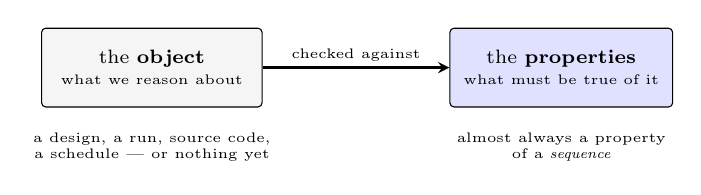
\begin{tikzpicture}[
  font=\scriptsize, >=stealth,
  b/.style={draw, rounded corners=1.5pt, align=center, inner sep=5pt,
            minimum height=1.0cm, minimum width=2.8cm},
  lab/.style={font=\tiny, align=center, inner sep=2pt}
]
  \node[b, fill=black!4]  (obj)  at (0,0)    {the {\bf object}\\{\tiny what we reason about}};
  \node[b, fill=blue!12]  (prop) at (5.2,0)  {the {\bf properties}\\{\tiny what must be true of it}};

  \node[lab, anchor=north] at (0,-0.75)   {a design, a run, source code,\\a schedule --- or nothing yet};
  \node[lab, anchor=north] at (5.2,-0.75) {almost always a property\\of a {\em sequence}};

  \draw[->, thick] (obj) -- node[font=\tiny, above, inner sep=2pt] {checked against} (prop);
\end{tikzpicture}\par}

\pause
\vspace{0.75cm}

Both must be written in a notation a machine can read.

\end{frame}

%----------------------------------------
\begin{frame}
  \frametitle{Five methods} \small

\vspace{-0.1cm}

\begin{center}\scriptsize
\renewcommand{\arraystretch}{1.25}
\setlength{\tabcolsep}{4pt}
\begin{tabular}{|>{\raggedright\arraybackslash}p{1.7cm}%
                |>{\raggedright\arraybackslash}p{2.1cm}%
                |>{\raggedright\arraybackslash}p{2.15cm}%
                |>{\raggedright\arraybackslash}p{2.4cm}|}
\hline
\rowcolor{blue!10}
{\bf Method} & {\bf Object} & {\bf Coverage} & {\bf Tools}\\
\hline
\rowcolor{orange!14}
\multicolumn{4}{|l|}{{\bf dynamic analysis} --- the system runs}\\
\hline
{\icontest[0.75]}\newline testing & the real system & one run per test & \ours{\fuzz{}}\\
\hline
{\iconrv[0.75]}\newline runtime verification & one real execution & that run, exactly & \ours{\tc{}, \daut{},
                                                                \pycontract{},
                                                                \dejavu{}}\\
\hline
\rowcolor{orange!14}
\multicolumn{4}{|l|}{{\bf static analysis} --- the system does not run}\\
\hline
{\iconcs[0.75]}\newline coding standards & source code & all runs, approximated & \comm{JPL checkers}\\
\hline
{\iconmc[0.75]}\newline model checking & a finite-state model & all runs of the {\em model} & \spin{},
                                                                     \tlaplus{},
                                                                     \ours{JPF1}\\
\hline
{\icontp[0.75]}\newline theorem proving & a mathematical model & all runs, unbounded & \lean{}, \zthree{},
                                                                     \esbmc{},
                                                                     \ours{\tasksat{}},
                                                                     \ours{\fcheck{}},
                                                                     \ours{\eva{}},
                                                                     \ours{K}\\
\hline
\end{tabular}
\end{center}

\vspace{-0.1cm}

\hfill {\scriptsize \ours{our tools} \quad \comm{commercial}}

\end{frame}
        %  2 min
%----------------------------------------
\begin{frame}
  \frametitle{Part 1}

\icontest[3.2]

\vspace{0.45cm}

{\Large\bf Testing: the execution does not exist yet}

\vspace{0.4cm}

{\small \fuzz{}, built on \matl{} and \zthree{}}

\end{frame}

%----------------------------------------
\begin{frame}
  \frametitle{Fuzzing a command-driven system} \small

\begin{figure}
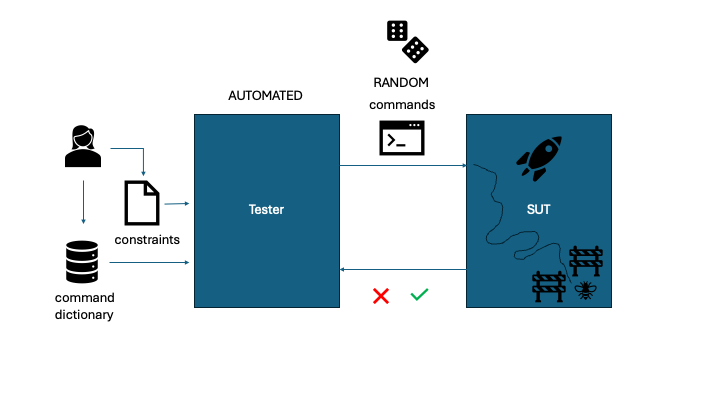
\includegraphics[width=0.62\textwidth]{figures/start5.png}
\end{figure}

Spacecraft are operated by {\bf sequences of commands}, tested by hand-written ones
that do not reach the corners. Random sequences do, but are rejected as illegal.

\pause
\vspace{0.15cm}

\begin{block}{}\small
\centering
So: {\bf constrain the randomness}. The user says what a legal sequence looks
like, in temporal logic; we generate random sequences satisfying it.
\end{block}

\end{frame}

%----------------------------------------
\begin{frame}[fragile]
  \frametitle{From temporal logic to a solver} \small

The specification language is {\bf \matl{}} --- temporal logic over events that
carry data, with binding. {\em Every sample collected is eventually downlinked}:
\[
\Box (\mathit{COLLECT}(file=f?) \Rightarrow \Diamond\, \mathit{SEND}(file=f))
\]

\pause
\vspace{-0.1cm}

A test is a function from position to command, and the formula becomes a constraint
on it. Writing $p$ for the {\tt COLLECT} and $q$ for the matching {\tt SEND},
unfolding over length 3:

\vspace{-0.2cm}

\begin{align*}
&\neg p(test(0)) \vee q(test(0)) \vee q(test(1)) \vee q(test(2)) \\
\wedge\quad &\neg p(test(1)) \vee q(test(1)) \vee q(test(2)) \\
\wedge\quad &\neg p(test(2)) \vee q(test(2))
\end{align*}

\vspace{-0.15cm}

\pause

Hand that to {\bf \zthree{}}, and a satisfying assignment {\em is} a legal test:

\begin{lstlisting}[language=python]
{'name': 'COLLECT', 'number': 1, 'time': 363, 'file': 'img042'}
{'name': 'COLLECT', 'number': 2, 'time': 373, 'file': 'log007'}
{'name': 'SEND',    'number': 3, 'time': 383, 'file': 'img042'}
{'name': 'SEND',    'number': 4, 'time': 394, 'file': 'log007'}
\end{lstlisting}

\vspace{-0.15cm}

Two collections outstanding at once, and {\em both} downlinked --- the binding on
$f$ is what makes that a real obligation rather than one \tool{SEND} satisfying
everything.

\end{frame}
       %  3 min   Part 1   testing
%----------------------------------------
\begin{frame}
  \frametitle{Part 2}

\iconrv[3.2]

\vspace{0.45cm}

{\Large\bf Runtime verification: one execution of the real thing}

\vspace{0.4cm}

{\small \tc{}, \logfire{}, \daut{}, \dejavu{}}

\end{frame}

%----------------------------------------
\begin{frame}
  \frametitle{The run you already have} \small

{\bf Instrument the code to emit events} --- or use what it already emits: telemetry,
command logs, event reports. Either way you have the thing we want to reason about: a
{\bf sequence of events}.

\vspace{0.35cm}

{\centering
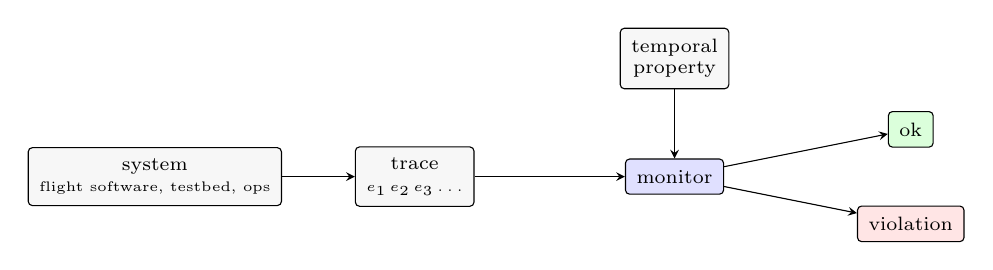
\begin{tikzpicture}[
  font=\scriptsize, >=stealth,
  b/.style={draw, rounded corners=1.5pt, align=center, inner sep=4pt, fill=black!3},
  lab/.style={font=\tiny, inner sep=1.5pt}
]
  \node[b] (sys) at (0,0)    {system\\{\tiny flight software, testbed, ops}};
  \node[b] (tr)  at (3.3,0)  {trace\\{\tiny $e_1\,e_2\,e_3\ldots$}};
  \node[b, fill=blue!12] (mon) at (6.6,0) {monitor};
  \node[b] (spec) at (6.6,1.5) {temporal\\property};
  \node[b, fill=green!14] (ok)  at (9.6,0.6)  {ok};
  \node[b, fill=red!10]   (bad) at (9.6,-0.6) {violation};

  \draw[->] (sys) -- (tr);
  \draw[->] (tr)  -- (mon);
  \draw[->] (spec) -- (mon);
  \draw[->] (mon) -- (ok);
  \draw[->] (mon) -- (bad);
\end{tikzpicture}\par}

\pause
\vspace{0.35cm}

No model to build and justify, and it scales to any system that can be made to
talk. The price: it says nothing about the runs you did not observe.

\end{frame}

%----------------------------------------
\begin{frame}[fragile]
  \frametitle{Writing monitors} \small

A monitor is an {\bf internal DSL} --- ordinary code in a host language, which
supplies the data handling for free. {\em Every dispatched command must eventually
succeed}, in \pycontract{}:

\begin{lstlisting}[language=python]
class Commands(Monitor):
    @initial
    class Start(AlwaysState):
        def transition(self, event):
            match event:
                case Dispatch(cmd, nr): return self.DoSucceed(cmd, nr)

    @data
    class DoSucceed(HotState):          # an obligation, not yet met
        cmd: str
        nr: int
        def transition(self, event):
            match event:
                case Succeed(self.cmd, self.nr): return ok
                case Fail(_, self.nr):  return error(f'{self.cmd} failed')
\end{lstlisting}

\pause

\ipromela{HotState} is the point: an obligation still {\em open} when the trace ends
is itself a violation. That is $\Box(p \rightarrow \Diamond q)$ with $nr$ bound ---
and the pattern matching is Python's, not ours.

\end{frame}

%----------------------------------------
\begin{frame}[fragile]
  \frametitle{\dejavu{}: an external DSL} \small

\dejavu{} goes the other way --- {\bf its own language}, not a host's. The same
obligation, turned into the past: {\em every command that succeeds was dispatched}.

\[
\forall c.\,\forall n.\ \mathit{succeed}(c,n) \rightarrow\;
\DDiamond\, \mathit{dispatch}(c,n)
\]

Fifteen lines of Python become one line of {\bf first-order past LTL} --- no state
machine, no bookkeeping of which pairs are outstanding. The quantifiers do it.

\pause
\vspace{0.3cm}

\begin{block}{}\small
\centering
Under the hood, {\bf BDDs} store the data --- which is what makes the monitoring
efficient.
\end{block}

\end{frame}

%----------------------------------------
\begin{frame}
  \frametitle{Five tools, and where they were used} \small

\begin{center}\scriptsize
\renewcommand{\arraystretch}{1.35}
\setlength{\tabcolsep}{4pt}
\begin{tabular}{|l|l|>{\raggedright\arraybackslash}p{2.35cm}%
                    |>{\raggedright\arraybackslash}p{2.1cm}%
                    |>{\raggedright\arraybackslash}p{2.1cm}|}
\hline
\rowcolor{blue!10}
& {\bf Host} & {\bf Formalism} & {\bf Engine} & {\bf Applied in}\\
\hline
\ours{\tc{}}         & Scala  & LTL + state machines    & formula rewriting       & \ladee{}\\
\hline
\ours{\logfire{}}    & Scala  & rules, facts in and out & Rete                    & \msl{}\\
\hline
\ours{\daut{}}       & Scala  & data automata           & indexed state machines  & \msnEndurance{}\\
\hline
\ours{\pycontract{}} & Python & data automata           & indexed state machines  & \msnEndurance{}
                                                                             \clipper{}\\
\hline
\ours{\dejavu{}}     & ---    & first-order past LTL    & BDDs over data          & ---\\
\hline
\end{tabular}
\end{center}


\end{frame}
             %  4 min   Part 2   runtime verification
%----------------------------------------
\begin{frame}
  \frametitle{Part 3}

\iconcs[3.2]

\vspace{0.45cm}

{\Large\bf Coding standards: rules a tool can decide}

\vspace{0.4cm}

{\small the cheapest row, and the one with the widest reach}

\end{frame}

%----------------------------------------
\begin{frame}
  \frametitle{Not everything worth doing is a model checker} \small

Crossing into static analysis --- no run at all, just the source.

\vspace{0.3cm}

In 2010--11: JPL's institutional {\bf Java coding standard} and the checker that
enforces it, and automated checking of the {\bf C, C++ and Java} standards across
the Lab.

\pause
\vspace{0.45cm}

\begin{block}{}\small
\centering
{\bf Applied and enforced on missions} --- institutionally, across flight projects.
\end{block}

\vspace{0.35cm}

\centering {\em Cannot check functional correctness --- does it do the right thing?}

\end{frame}
       %  1 min   Part 3   coding standards
%----------------------------------------
\begin{frame}
  \frametitle{Part 4}

\iconmc[3.2]

\vspace{0.45cm}

{\Large\bf Model checking: all executions of a design}

\vspace{0.4cm}

{\small \spin{}, and \ours{\jpf{} 1 (JPF1)}}

\end{frame}

%----------------------------------------
\begin{frame}
  \frametitle{The Deep Space 1 Remote Agent, 1999} \small

First autonomous control of a NASA spacecraft. We analyzed the executive's locking
layer: {\bf 3000 lines} of multithreaded Lisp, hand-translated to {\bf 500 lines} of
\promelaname{} --- twelve man-weeks. {\bf Five} flawed fragments, all real.

\pause
\vspace{0.3cm}

\begin{block}{}\small
Then, in flight, 96 million kilometres out: {\bf thrusting did not turn off when
requested}. A deadlock --- a missing critical section around a conditional wait. {\bf
The same defect \spin{} had already found}, in code {\bf copied} into another module
with the critical section left out. That module was never analyzed.
\end{block}

\end{frame}

%----------------------------------------
\begin{frame}[fragile]
  \frametitle{A lock-free priority queue, August 2026} \small

Callable from an interrupt handler, so: no mutex, compare-and-swap instead --- plus a
counter \tool{avail} so a consumer can skip the scan.

\begin{lstlisting}[style=shell]
send(m):     claim FREE slot; write; publish; avail += 1
receive():   if avail == 0: return EMPTY        # peek the counter
             m = getMessage()                  # scan, CAS a READY slot
             if m == empty: return EMPTY
             avail -= 1                        # count down
             return m
\end{lstlisting}

\pause

Two producers, two consumers, two slots; of a slot, only its {\bf state}. \spin{}:

\begin{lstlisting}[style=shellhl]
pan:1: assertion violated (avail>=0) (at depth 11)
  P  publish slot 0, avail++                       avail = 1
  C1 peek: avail > 0, pass    C2 peek: avail > 0, pass
  C1 getMessage -> slot 0, avail--                 avail = 0
(*\hlon\ttfamily\ \ P\ \ publish slot 1 -{}- but avail++ not yet\hloff*)
  C2 getMessage -> slot 1, avail--                 avail = -1
\end{lstlisting}

Both consumers got a message, from {\em different} slots, so both counted down ---
but only one \tool{avail++} had landed. The field is \tool{unsigned}: telemetry reads
{\bf 4\,294\,967\,295}.

\pause

{\bf The fix:} \tool{avail++} {\em before} publishing. \tool{1992 states, errors: 0}.

\end{frame}
  %  5 min   Part 4   model checking
%----------------------------------------
\begin{frame}
  \frametitle{Part 5}

\icontp[3.2]

\vspace{0.45cm}

{\Large\bf Theorem proving: all executions, no bound}

\vspace{0.4cm}

{\small \ours{\fcheck{}} using \lean{} 4, \ours{\tasksat{}} using \zthree{},\\[0.2cm]
\ours{\esbmcpy{}} using \esbmc{}}

\end{frame}

%----------------------------------------
\begin{frame}[fragile]
  \frametitle{\fcheck{}: proving an \fprime{} application} \small

\newtag{} \ {\bf \fcheck{}} --- a {\em new} tool of ours, using \lean{} 4. The
hysteresis logic of {\tt HeaterController}, in flight C++:

\begin{lstlisting}[style=cpp]
if (m_controlMode != ControlMode::AUTOMATIC) return;
HeaterState newState = m_heaterState;
if      (avgTemp < (m_targetTemp - m_hysteresis)) newState = ON;
else if (avgTemp > (m_targetTemp + m_hysteresis)) newState = OFF;
if (newState != m_heaterState) commandHeater(newState);
\end{lstlisting}

\vspace{-0.15cm}

and the \lean{} model --- \iconllm[0.85]\ {\bf LLM-generated} --- tracking it line
for line:

\begin{lstlisting}[language=lean4]
def avgTempIn_handler (s : ControllerState) (d : AvgTempData) :=
  if s.controlMode != ControlMode.AUTOMATIC then s
  else let newState :=
    if d.avgTemp < s.targetTemp - s.hysteresis then ON
    else if d.avgTemp > s.targetTemp + s.hysteresis then OFF
    else s.heaterState
  if newState != s.heaterState then commandHeater s newState else s
\end{lstlisting}

\end{frame}

%----------------------------------------
\begin{frame}[fragile]
  \frametitle{\fcheck{}: what the proof attempt found} \small

\begin{lstlisting}[language=lean4]
theorem cold_reading_turns_heater_on (s) (d)
    (ha    : s.controlMode = ControlMode.AUTOMATIC)
    (hcold : d.avgTemp < s.targetTemp - s.hysteresis) :
    (avgTempIn_handler s d).heaterState = HeaterState.ON
\end{lstlisting}

Too cold $\Rightarrow$ heater ON, for {\em every} state and {\em every} reading.

\pause
\vspace{0.4cm}

\begin{block}{Arbitrary operator behaviour}\small
\begin{lstlisting}[language=lean4]
theorem executeTrace_preserves_invariant
    (sys) (trace : List SystemEvent)
    (hInv : SystemInvariant sys) :
    SystemInvariant (executeTrace sys trace)
\end{lstlisting}
{\scriptsize No sequence of commands and ticks --- of {\em any} length --- can break the
invariant. \spin{} would have had to bound that list.}
\end{block}

\end{frame}

%----------------------------------------
\begin{frame}[fragile]
  \frametitle{\tasksat{}: proof without a proof script} \small

\newtag{} \ a {\em new} tool for {\bf planning and scheduling}, inspired by MEXEC.
A {\bf task net} declares timelines --- states, resources, rates --- and tasks with
windows, preconditions and impacts:

\begin{lstlisting}[language=tasknetdsl,frame=single]
  battery : rate [10.0, 100.0] bounds [0.0, 100.0] = 60.0;

  task drive {
    startrange [100, 120];  durationrange [30, 40];
    pre     { battery in [60.0, 100.0]; }
    impacts { maint { battery +~ -1.5; }  post { location = target; } }
  }

  constraints { always not (active(charge) and active(drive)); }
  properties  { eventually (location = target and data >= 30); }
\end{lstlisting}

\pause

\begin{block}{Two problems, one encoding}\small
\[
\text{schedule:}\quad \exists\, \mathit{init}.\ \exists\, \mathit{sched}.\ C(\mathit{init},\mathit{sched})
\qquad
\text{verify:}\quad \forall\, \mathit{init}.\ \forall\, \mathit{sched}.\ C \rightarrow \varphi
\]
\end{block}

Flip one quantifier and the planner becomes a {\bf prover} --- discharged
symbolically, for {\em every} initial battery level and start time, not a state graph.

\end{frame}

%----------------------------------------
\begin{frame}
  \frametitle{\esbmcpy{}: verifying Python} \small

\newtag{} \ Why Python: we are building a {\bf Python model of an autonomous system}
in the {\bf PAAS} project. And Python has no model checker of the kind \spin{} is ---
so {\bf translate it into something that does}, and let \esbmc{} decide.

\vspace{0.35cm}

{\centering
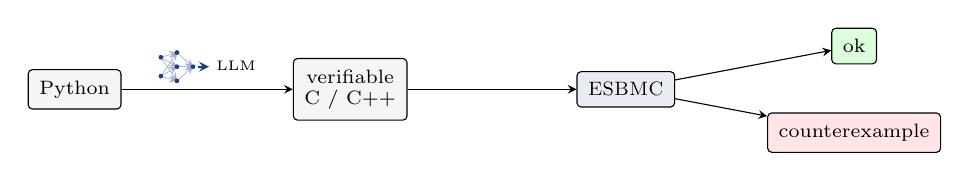
\begin{tikzpicture}[
  font=\scriptsize, >=stealth,
  b/.style={draw, rounded corners=1.5pt, align=center, inner sep=4pt, fill=black!4},
  lab/.style={font=\tiny, inner sep=2pt}
]
  \node[b] (py)  at (0,0)    {Python};
  \node[b] (c)   at (3.5,0)  {verifiable\\C / C++};
  \node[b, fill=iconcol!10] (e) at (7.0,0) {\esbmc{}};
  \node[b, fill=green!14] (ok)  at (9.9,0.55)  {ok};
  \node[b, fill=red!10]   (bad) at (9.9,-0.55) {counterexample};

  \draw[->] (py) -- node[lab, above] {\iconllm[0.6]\ LLM} (c);
  \draw[->] (c)  -- (e);
  \draw[->] (e)  -- (ok);
  \draw[->] (e)  -- (bad);
\end{tikzpicture}\par}

\vspace{0.35cm}

Three routes to the C: {\bf Shedskin} for what converts statically, an {\bf LLM} for
what does not, and {\bf dynamic tracing} for what neither can reach.

\vspace{0.2cm}

Driving it: \ours{\eva{}}, the {\bf Enhanced Verification Agent} --- which also runs
the static analysers and the runtime checks, and iterates.

\vspace{0.2cm}

\begin{block}{}\small
\centering
The LLM does the translating. \esbmc{} does the deciding.
\end{block}

\vspace{0.25cm}

{\scriptsize Largely developed by GenAI and the University of Manchester.}

\end{frame}
           %  4 min   Part 5   theorem proving
%----------------------------------------
\begin{frame}
  \frametitle{Part 6}

\iconllm[3.2]

\vspace{0.45cm}

{\Large\bf LLMs: writing the model was always the expensive part}

\end{frame}

%----------------------------------------
\begin{frame}
  \frametitle{Who wrote the queue model?} \small

Twelve man-weeks for the Remote Agent model. That cost --- not the checking --- is
why formal methods stayed a specialist activity.

\pause
\vspace{0.3cm}

The lock-free queue in Part 4 went differently. An LLM reading the pull request
{\bf flagged} the counter as suspicious; asked to demonstrate it, it {\bf wrote the
\promelaname{} model}. \spin{} then did what \spin{} does.

\vspace{0.4cm}

{\centering
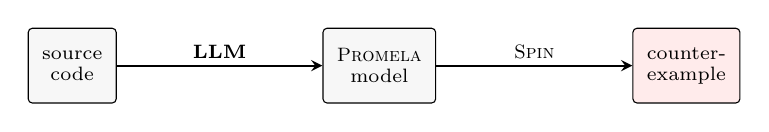
\begin{tikzpicture}[
  font=\scriptsize, >=stealth,
  box/.style={draw, rounded corners=1.5pt, align=center, inner sep=5pt,
              minimum height=0.95cm, fill=black!3},
  lab/.style={font=\scriptsize\bfseries, inner sep=2pt}
]
  \node[box] (code)  at (0,0)    {source\\code};
  \node[box] (model) at (3.9,0)  {\promelaname{}\\model};
  \node[box, fill=red!8] (cex) at (7.8,0) {counter-\\example};

  \draw[->, thick] (code)  -- node[lab, above] {LLM}    (model);
  \draw[->, thick] (model) -- node[lab, above] {\spin{}} (cex);
\end{tikzpicture}\par}

\pause
\vspace{0.3cm}

\begin{block}{}\small
\centering
The LLM proposes. The model checker disposes.
\end{block}

An LLM asserting that code is correct is worth little. An LLM producing an
artifact that a {\bf sound tool} then checks is worth a great deal --- and if the
model is wrong, the counterexample is concrete enough to see that it is wrong.

\end{frame}
            %  3 min   Part 6   LLMs
%%----------------------------------------
\begin{frame}
  \frametitle{What thirty years suggests} \small

\begin{itemize}
\item {\bf Write the property down.} Most of the value arrives before any tool
      runs. Every project above started with someone stating, precisely, what must
      be true --- and the two DS1 properties were written by the programmers, not
      by us.

\pause
\item {\bf Temporal logic is the common currency.} The same $\Box(p \rightarrow
      \Diamond q)$ was checked over all executions of a model, over one telemetry
      stream, and over a test that did not exist yet.

\item {\bf Pick the method to fit the object you have.} A design and no code:
      model checking. A running system and a log: runtime verification. Source and
      nothing else: static analysis. A guarantee that must hold for unbounded runs:
      proof. No object at all, and you need a test or a schedule: constraint solving.

\pause
\item {\bf The bottleneck was always the model, never the checker.} That is
      exactly the bottleneck LLMs now attack --- with the sound tool still doing
      the deciding.

\pause
\item {\bf Concurrency is where this pays.} Testing samples one interleaving.
      Every defect in this talk lived in the gap between a check and the act that
      depended on it.
\end{itemize}

\end{frame}
    %  takeaways --- dropped, file kept on disk
%----------------------------------------
\begin{frame}
  \frametitle{The LLM writes the object --- for every one of them} \small

\vspace{-0.1cm}

{\centering
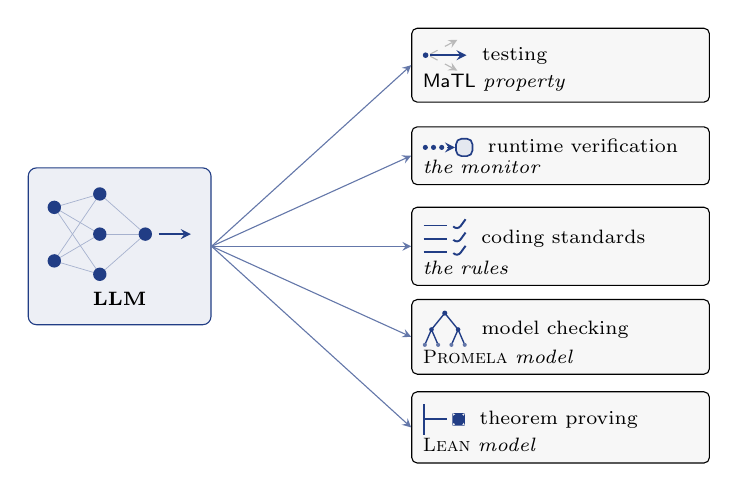
\begin{tikzpicture}[
  font=\scriptsize, >=stealth,
  m/.style={draw, rounded corners=2pt, align=left, inner sep=4pt, fill=black!3,
            text width=3.5cm},
  llm/.style={draw=iconcol, rounded corners=3pt, fill=iconcol!8, align=center,
              inner sep=7pt}
]
  \node[llm] (llm) at (0,0) {\iconllm[1.7]\\[3pt]{\bf LLM}};

  \node[m] (a) at (5.6, 2.30) {\icontest[0.65]\ \ testing\\{\em \matl{} property}};
  \node[m] (b) at (5.6, 1.15) {\iconrv[0.65]\ \ runtime verification\\{\em the monitor}};
  \node[m] (c) at (5.6, 0.00) {\iconcs[0.65]\ \ coding standards\\{\em the rules}};
  \node[m] (d) at (5.6,-1.15) {\iconmc[0.65]\ \ model checking\\{\em \promelaname{} model}};
  \node[m] (e) at (5.6,-2.30) {\icontp[0.65]\ \ theorem proving\\{\em \lean{} model}};

  \foreach \n in {a,b,c,d,e} { \draw[->, iconcol!70] (llm.east) -- (\n.west); }
\end{tikzpicture}\par}

\vspace{0.15cm}

\begin{block}{}\small
\centering
The LLM proposes the {\bf object}. The sound tool still disposes.
\end{block}

\vspace{0.3cm}

\centering {\Large\bf Questions?}

\end{frame}
      %  --

\end{document}
